\documentclass{class}
\usepackage{multicol}
\usepackage{float}
\usepackage{graphicx}
\usepackage{tabularx}
\usepackage{array}
\usepackage{caption}
\usepackage{enumitem} % Customize bullet lists
\usepackage{listings} % Code listings

%% Abbreviated author list for the running footer
\bibliography{References}

\abstract{prova}
\keywords{Big Data • Hadoop • Spark • ML • MongoDB • Data Analysis • Data Visualization • Python}
% Publication Title
\title{From Raw Data to Informed Decisions:\\ Analyzing Amazon Book Reviews}
% Short title for the header (copy the main title if it is not too long)
\shorttitle{Analysis of Amazon Book Reviews}

% Authors
\author[1]{Alberti A.,Ligari D., Andreoli A.}
% Author Affiliations
\affil[1]{Data Science and Big data Analytics course, University of Pavia, Department of Computer Engineering (Data Science), Pavia, Italy}
% Surname of the first author of the manuscript
\firstauthor{Ligari, Alberti, Andreoli}
% Publication data (will be defined in the edition)
\publicationdate{\today}
% Place your particular definitions here
\newcommand{\vect}[1]{\mathbf{#1}}  % vectors
\github{https://github.com/DavideLigari01/data-science-project}

\begin{document}

\maketitle

\tableofcontents

\thispagestyle{FirstPage}

\section{Introduction}
\firstword{I}{n}
the age of digital commerce, customer reviews profoundly impact product perception and purchase decisions.
Amazon, with its extensive repository of book reviews spanning nearly two decades, holds a wealth of valuable insights,
sentiments, and trends. This project aims to create a scalable solution for uncovering patterns, sentiment trends,
and correlations within the realm of book reviews, utilizing advanced tools and technologies.\\
In this report, we provide a detailed exploration of our project, covering stages from initial data discovery
and preparation to feature extraction, model building, and evaluation.

\section{Discovery}

\subsection*{Team}
\subsection*{Tools}
\subsection*{Framing}
\section{Data Preparation}
\subsection*{Data Collection}
\subsection*{Hypothesis Generation}
\subsection*{Data Cleaning}
\pagestyle{OtherPage}

\subsection*{Data aggregation}

The MapReduce job was created to perform the inner join operation on the "Data table" and the "Rating table" based on the title.
The output of the MapReduce job is a single file containing the joined records from both tables.

\subsubsection*{Mapper}
The Mapper script processes the input data line by line, where each line represents a distinct record.
It transforms these lines into a key-value structure, where the key corresponds to the book title, and
the value contains the remaining content of the line.\\
Given that the Mapper deals with data from two distinct sources,
it becomes crucial to distinguish between records belonging to the 'Data table' and those in the 'Rating table'.
This distinction is essential because it mandates a specific order of processing records from the 'Data'
table need to be joined with corresponding records from the 'Rating' table in the Reducer phase.
Consequently, the Reducer should process 'Data' table records before 'Rating' table records.
To ensure this orderly processing, the Mapper augments the key with a special character for each table type.
Specifically, it appends a hyphen ('-') as the second key element for records from the 'Data table' and 'www'
for records from the 'Rating table.'
By doing so, and thanks to Hadoop's sorting task made after, the Mapper guarantees that 'Data table' records are encountered
and processed prior to 'Rating table' records during the subsequent phases of MapReduce.

\subsubsection*{Reducer}

The Reducer script is responsible for processing the intermediate output records generated by the Mapper.
Its primary role is to perform the join operation between the 'Data' table and the 'Rating' table,
taking advantage of the pre-sorting of records by title.
During its execution, the Reducer reads the records in a sequential order.
As it encounters a record from the 'Data' table, it stores the information in one variable.
Conversely, when it comes across a record from the 'Rating' table, it stores that information in another variable.
Once both 'Data' and 'Rating' records for the same title are available,
the Reducer performs the join operation by combining the data from these records.

\subsection*{MongoDB loading}
\section{Local Hypotheses Testing}
\subsection*{Hypothesis 1}

\textbf{H0 (Null Hypothesis):} There is a positive correlation between the length of a review and its helpfulness score.\\
\noindent
The data cleaning and 'review/helpfulness' transformation process ($\text{helpfulness score} = \frac{x}{y} \sqrt{y}$) was executed using the `pymongo` library to leverage the efficiency of MongoDB. 
Specifically, we designed a pipeline to perform the necessary operations. Regarding the 'review/text' transformation, we employed the `nltk` 
library to tokenize the text, remove punctuation, stopwords, and subsequently count the number of words.\\
The correlation coefficient between the two variables is 0.3313 with a p-value < 0.05, indicating a statistically significant correlation.
A graphical representation confirming this correlation can be found in Figure \ref{fig:h1_boxplot}. There is a positive correlation observed until 
approximately 400 words, beyond which the boxplot stabilizes. Consequently, we conducted an analysis of the correlation within specific review length 
groups. As a result (Table \ref{corr_groups}), we observed a positive and statistically significant correlation for reviews with lengths between 0 and 400 words. 
However, for reviews longer than 750 words, the correlation becomes negative and statistically significant. For reviews falling in the intermediate range 
(between 400 and 750 words), the correlation is negligible.
\noindent
\textbf{Conclusion:} The hypothesis is confirmed, but the correlation is not very strong and varies depending on the length of the review.

\begin{figure}[H]
    \centering
    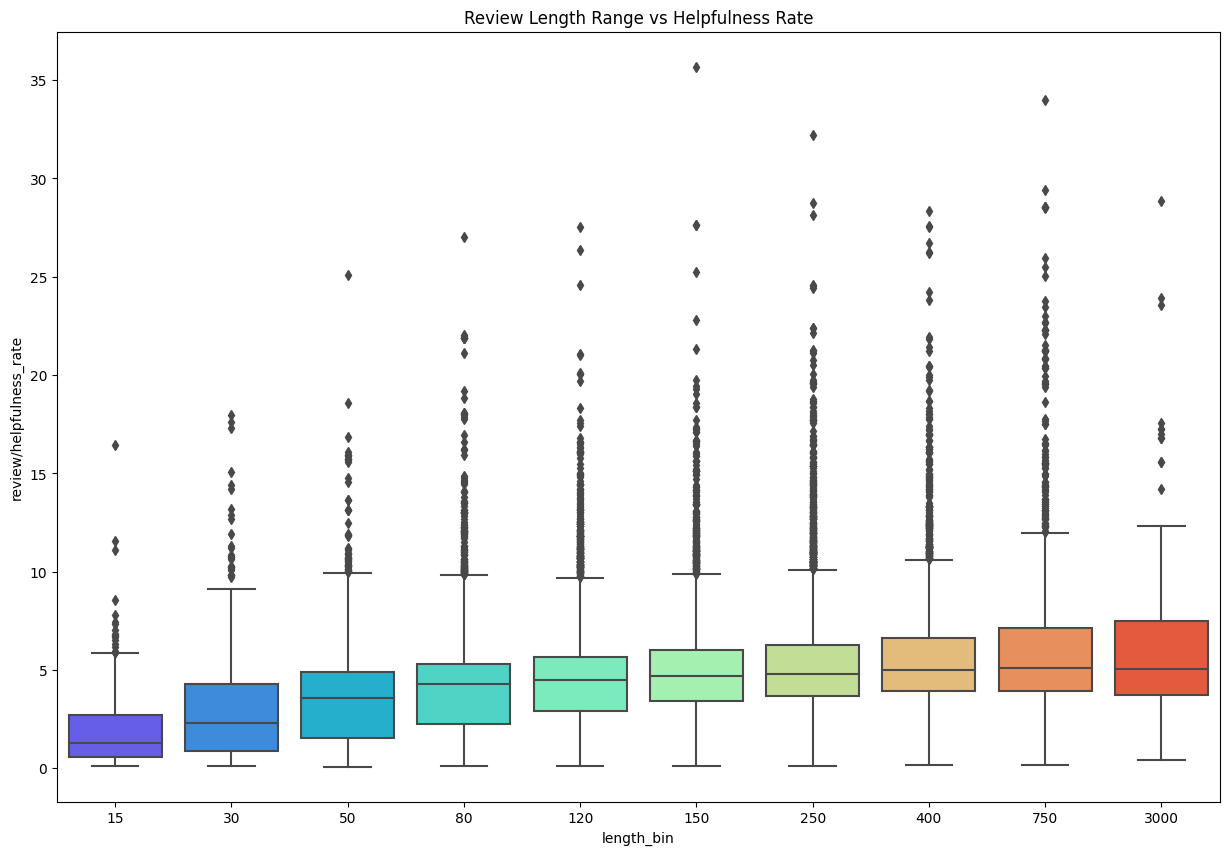
\includegraphics[width=0.49\textwidth]{./figures/h1_boxplot.png}
    \caption{Correlation between review length and helpfulness score for different review length groups}
    \label{fig:h1_boxplot}
\end{figure}

\begin{table}[H]
    \footnotesize
    \centering
    \caption{Correlation Coefficients and P-values for Different Groups}
    \begin{tabular}{|c|c|c|}
    \hline
    Group Number & Correlation Coefficient & P-value \\
    \hline
    400 & 0.2216 & 0.0000 \\
    \hline
    750 & -0.0188 & 0.2585 \\
    \hline
    3000 & -0.1418 & 0.0065 \\
    \hline
    \end{tabular}
    \label{corr_groups}
\end{table}


\subsection*{Hypothesis 2}
\subsection*{Hypothesis 3}

\textbf{H0 (Null Hypothesis):} There is no correlation between the rating of a review and its helpfulness score.\\
\noindent
Similar to the previous hypothesis, we addressed missing values and data transformations directly with a MongoDB query.
With the data prepared for analysis, we conducted an initial examination of the distribution of votes across the four rating
categories. Figure \ref{fig:h3_votes_distribution} reveals a \textbf{positive bias} where individuals tend to vote more for
positive reviews than negative ones. Specifically, a significant portion of votes for rating 5 consists of reviews with a
total vote count equal to 1. This introduces bias into our results because, based on the formula used to compute the
helpfulness score, a small total vote count would lead to a low helpfulness score. To mitigate this, we retained only
reviews with a total vote count greater than 20.

\begin{figure}[H]
    \centering
    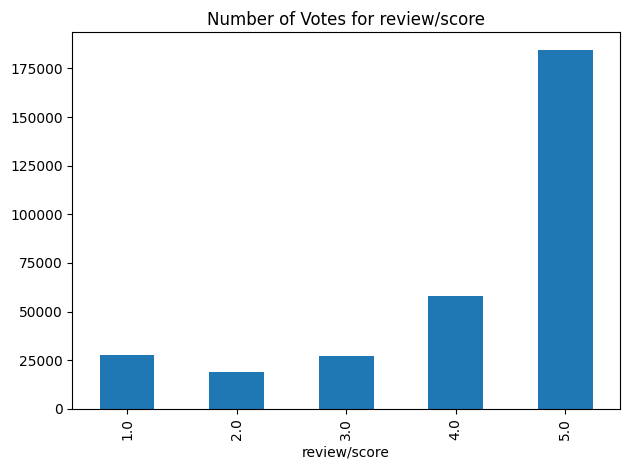
\includegraphics[width=0.4\textwidth]{./figures/h3_votes_distribution.png}
    \caption{Distribution of votes across the four rating categories}
    \label{fig:h3_votes_distribution}
\end{figure}

\noindent
The Spearman correlation coefficient between the two variables is $0.5247$, with a p-value of $0.0$.\\
\textbf{Conclusion:}
The hypothesis is confirmed as there is a positive and statistically significant correlation between the review rating
and helpfulness score. This finding is further supported by the boxplot in Figure \ref{fig:h3_boxplot}.

\begin{figure}[H]
    \centering
    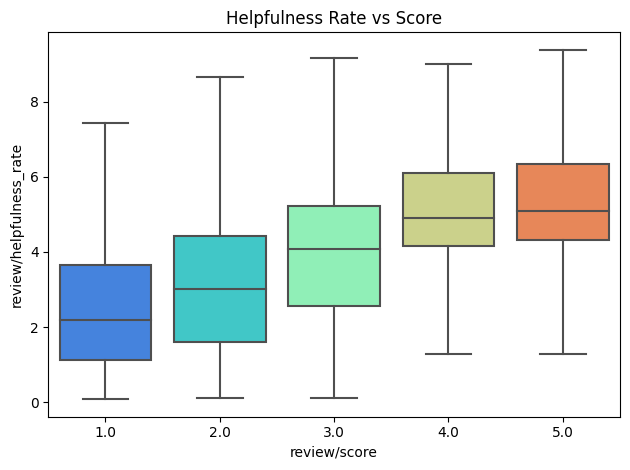
\includegraphics[width=0.3\textwidth]{./figures/h3_boxplot.png}
    \caption{Boxplot illustrating the correlation between review rating and helpfulness score}
    \label{fig:h3_boxplot}
\end{figure}

\subsection*{Hypothesis 4}
\subsection*{Hypothesis 5}
\subsection*{Hypothesis 6}

- The larger the number of books published for a category, the higher the review score.\\ 
- The larger the number of books published by publishers, the higher the review score.\\
\noindent
\textbf{Metric:} Correlation Coefficient.\\
\noindent
\textbf{Missing Values:}
\begin{itemize}
\item \textit{`publisher`:} remove the entire sample
\item \textit{`review/score`:} remove the entire sample
\item \textit{`categories`:} remove the entire sample
\end{itemize}
\noindent
\textbf{Data Transformation:}
\begin{itemize}
    \item \textit{`categories`:} GroupBy categories.
    \item \textit{`publisher`:} GroupBy publisher.
    \item \textit{`review/score`:} Compute the average review/score for each publisher and category.
\end{itemize}\vspace{0.5cm}
\noindent
\textbf{Description and Results}
All the data cleaning and transformation steps were performed using MongoDB with the aggregation pipeline, to have a more efficient and faster computation.\\
Specifically the data cleaning steps were performed using the \textit{\$match} operator, while the data transformation steps were performed using the \textit{\$group} operator with \textit{\$avg} operation.
Finally a \textit{\$project} operator was used to select the fields of interest. To reduce bias, we removed the categories having less than 50 books and the publishers having less than 20 books.\\
The results are shown in Table \ref{tab:h6_correlations}.\\
\textbf{Conclusion:} The hypotheses are falsified since the metrics shows no correlation between the two variables in both cases.

\begin{table}[H]
    \centering
    \caption{Correlation Values and P-values for Categories and Publishers}
    \begin{tabular}{|c|c|c|}
    \hline
    \textbf{Variable} & \textbf{Correlation Value} & \textbf{P-value} \\
    \hline
    Category & -0.0806 & 0.558 \\
    \hline
    Publisher & -0.0673 & 0.151 \\
    \hline
    \end{tabular}
    \label{tab:h6_correlations}
\end{table}

\vspace{0.5cm}
\noindent 
\textbf{Curiosity}
We performed two complex MongoDB queries (reported as example in section 'Code') to answer to two questions:\\
\begin{itemize}
    \item Which are the best publishers? (i.e. capable of getting avg scores above 4.5 in lots of categories)
    \item In which categories are the best publishers focused?
\end{itemize}

The results are reported in Figure \ref{fig:h6_which_best} and Figure \ref{fig:h6_where_best}.

\begin{figure}[H]
    \centering
    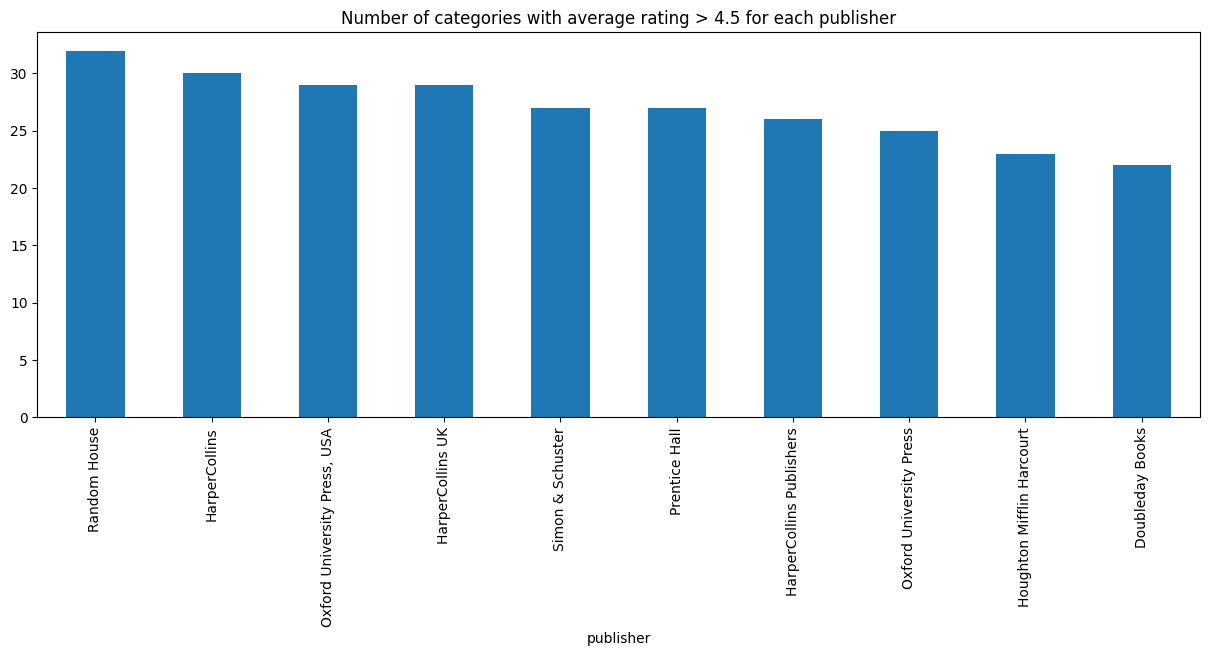
\includegraphics[width=0.5\textwidth]{./figures/h6_which_best.png}
    \caption{Which are the best publishers?}
    \label{fig:h6_which_best}
\end{figure}

\begin{figure}[H]
    \centering
    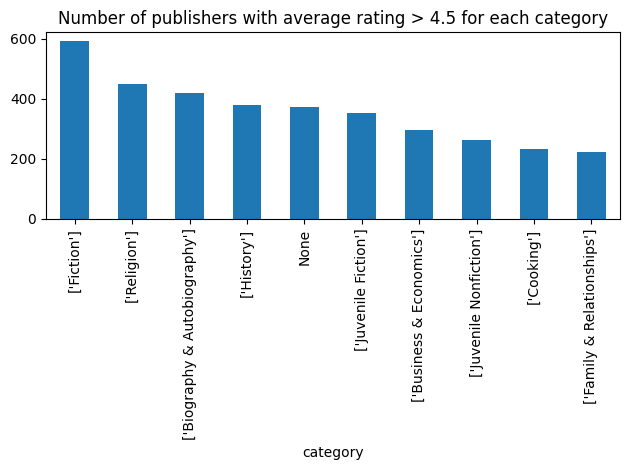
\includegraphics[width=0.5\textwidth]{./figures/h6_where_best.png}
    \caption{In which categories are the best publishers focused?}
    \label{fig:h6_where_best}
\end{figure}
\section{Spark Hypotheses Testing}
\section{Helpfulness Prediction}
\section{Conclusions}

%% Complex MongoDB query to answer: In which categories are the best publishers focused?

\section{Python Script}
\vspace{0.5cm}
This is the script to answer the question: In which categories are the best publishers focused?\\
\lstset{
    language=Python,
    basicstyle=\footnotesize\ttfamily,
    numbers=left,
    numberstyle=\tiny,
    numbersep=5pt
}

\begin{lstlisting}
# Deal with missing values
pipeline_missing = {'$match': {
    'review/score': {'$exists': True, '$ne': 0},
    'publisher': {'$exists': True, '$ne': None},
    'categories': {'$exists': True},
}
}

# Compute average rating for each tuple category, publisher
pipeline_average_rating = {'$group': {
    '_id': {
        'category': '$categories',
        'publisher': '$publisher',
    },
    'avg_score': {'$avg': '$review/score'},
    'count': {'$sum': 1}
}
}

# Show average rating for category for each publisher
pipeline_publisher = {'$group': {
    '_id': '$_id.category',
    'avg_score/publisher': {
        '$push': {
            'publisher': '$_id.publisher',
            'avg_score': '$avg_score',
            'count': '$count'
        }
    }
}
}

# Unwind the list of categories
pipeline_unwind = {'$unwind': '$avg_score/publisher'}

# Remove categories or publisher with less than 'threshold' reviews
threshold = 0
pipeline_remove = {'$match': {
    'avg_score/publisher.count': {'$gte': threshold}
}
}

# Count the number of categories with average rating > 4.5
pipeline_counts = {'$project': {
    'category': '$_id',
    '_id': 0,
    'publisher': '$avg_score/publisher.publisher',
    'count': {
        '$sum': {
            '$cond': {

                'if': {'$gt': ['$avg_score/publisher.avg_score', 4.5]},
                'then': 1,
                'else': 0
            }
        }
    }
}
}

# Sum the results for each publisher. If Total > 10, then the hypothesis is False
pipeline_sum = {'$group': {
    '_id': '$category',
    'total': {'$sum': '$count'}
}
}

pipeline_sort = {'$sort': {
    'total': -1
}
}

results = books.aggregate([pipeline_missing, pipeline_average_rating, pipeline_publisher,
                          pipeline_unwind, pipeline_remove, pipeline_counts,
                          pipeline_sum, pipeline_sort])
\end{lstlisting}




    

\end{document}
